% Created 2019-07-18 Thu 10:33
% Intended LaTeX compiler: pdflatex
\documentclass[presentation]{beamer}
\usepackage[utf8x]{inputenc}
\usepackage[T1]{fontenc}
\usepackage{graphicx}
\usepackage{grffile}
\usepackage{longtable}
\usepackage{wrapfig}
\usepackage{rotating}
\usepackage[normalem]{ulem}
\usepackage{amsmath}
\usepackage{textcomp}
\usepackage{amssymb}
\usepackage{capt-of}
\usepackage{hyperref}
\usetheme{Madrid}
\author{Billal Boudjoghra}
\date{\today}
\title{Projet de mémoire}
\subtitle{Détection des replays dans les vidéos de sport}
\setbeamertemplate{footline}[frame number author] \setbeamertemplate{caption}[numbered] \beamertemplatenavigationsymbolsempty \frametitle{} \useoutertheme{miniframes}
\hypersetup{
 pdfauthor={Billal Boudjoghra},
 pdftitle={Projet de mémoire},
 pdfkeywords={},
 pdfsubject={},
 pdfcreator={Emacs 26.2 (Org mode 9.1.9)}, 
 pdflang={English}}
\begin{document}

\maketitle
\begin{frame}{Outline}
\tableofcontents
\end{frame}


\section{Introduction}
\label{sec:org4ed27ed}
\begin{frame}[label={sec:org48b718a}]{Sportagraph : Présentation}
\begin{itemize}
\item son produit : Digital Asset Manager
\item mon poste : développeur Scala
\item ma tâche : détections des replays dans les vidéos de sport
\end{itemize}
\end{frame}

\begin{frame}[label={sec:org19d0132}]{Sujet de recherche : Détection des replays dans les vidéos de sport}
\begin{itemize}
\item en lien avec mon travail en entreprise
\item thème vaste : deep learning / computer vision
\end{itemize}
\end{frame}

\begin{frame}[label={sec:org410eea3}]{Détections des replays}
\begin{itemize}
\item Les replays sont les moments forts de la vidéo
\item Hypothèse : les replays sont compris entre deux logos
\item Objectif : détection/reconnaissance des logos
\end{itemize}
\begin{figure}[htbp]
\centering
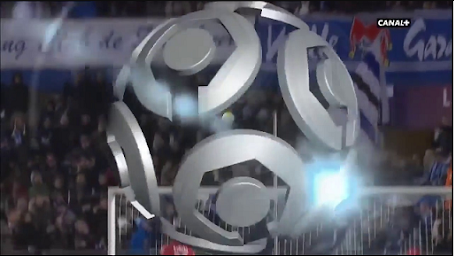
\includegraphics[width=5cm]{logo_ex.png}
\caption{Un logo}
\end{figure}
\end{frame}

\section{Détection par analyse d'image}
\label{sec:org04ef24c}
\begin{frame}[label={sec:orgce105de}]{ORB (1/3)}
\begin{itemize}
\item outil : OpenCV
\end{itemize}
\begin{block}{Idée}
\begin{itemize}
\item obtenir des features pour chaque frame de la vidéo (SIFT, ORB)
\item appliquer des algorithmes de machine learning sur ces features (K-NN)
\end{itemize}
\end{block}
\end{frame}

\begin{frame}[label={sec:org43dcfca}]{ORB (2/2)}
\begin{center}
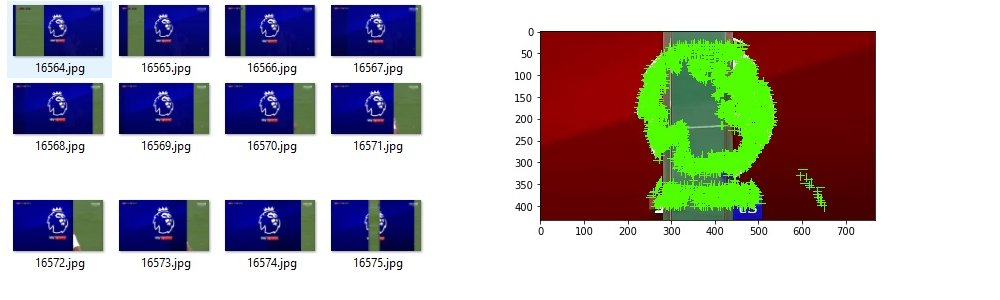
\includegraphics[width=.9\linewidth]{akaze_window_res2.jpg}
\end{center}
\end{frame}

\begin{frame}[label={sec:orgee2a7ca}]{ORB : Résultats (3/3)}
\begin{center}
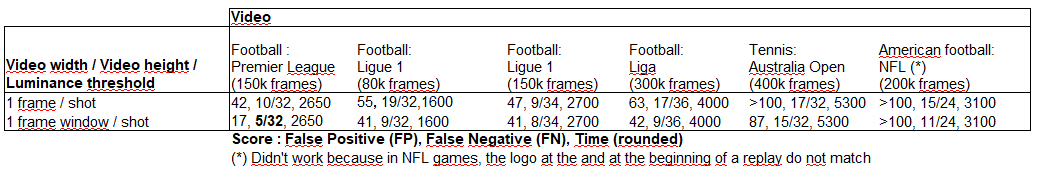
\includegraphics[width=12cm]{res_orb.png}
\end{center}
\end{frame}

\begin{frame}[label={sec:org5f2ad5f}]{Détection de contours (1/3)}
\begin{itemize}
\item outil : OpenCV
\end{itemize}
\begin{block}{Idée}
\begin{itemize}
\item détecter les contours pour chaque frame de la vidéo (canny edge detection)
\item logo image fixe => les contours des frames logo sont les mêmes
\end{itemize}
\end{block}
\end{frame}

\begin{frame}[label={sec:org4b309cd}]{Détection de contours (2/3)}
\begin{center}
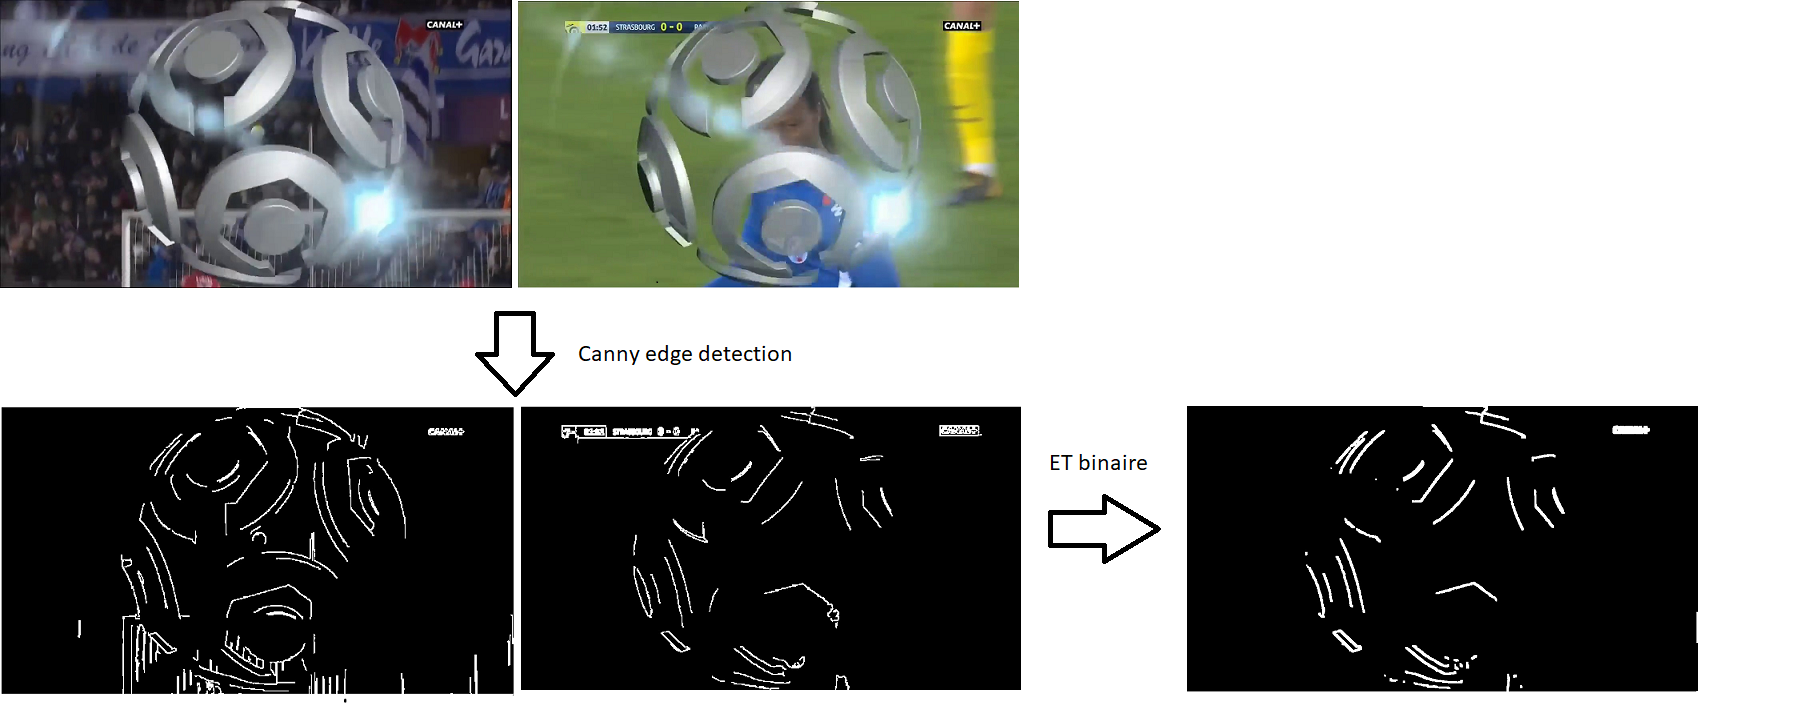
\includegraphics[width=.9\linewidth]{comparison_idea.png}
\end{center}
\end{frame}

\begin{frame}[label={sec:orgd30f5ed}]{Détection de contours : Résultats (3/3)}
\begin{center}
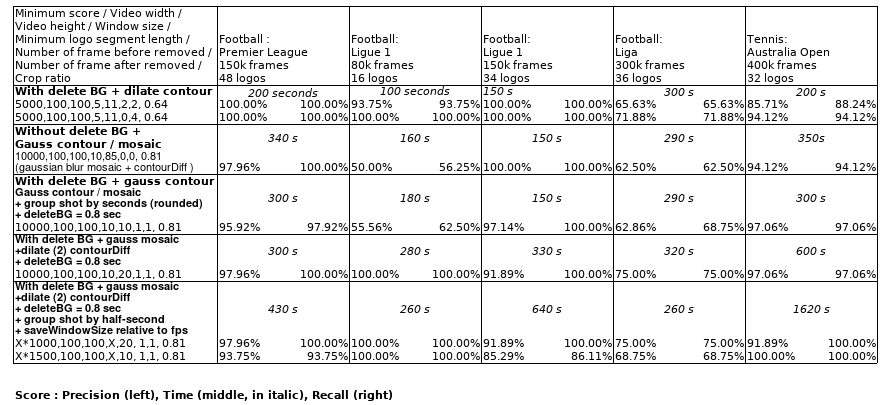
\includegraphics[width=.9\linewidth]{res_match_contour.png}
\end{center}
\end{frame}

\section{Réseau à convolution}
\label{sec:orgbca906d}
\begin{frame}[label={sec:orgc4f6df9}]{CNN}
\begin{itemize}
\item efficace pour la reconnaisance d'image
\item utilise la convolution au lieu de la multiplication matricielle
\item deux caractéristiques importantes : l'intéraction parcimonieuse et le partage de paramètres
\end{itemize}
\end{frame}

\begin{frame}[label={sec:org3e5b15f}]{CNN : opération de convolution}
\begin{figure}[htbp]
\centering
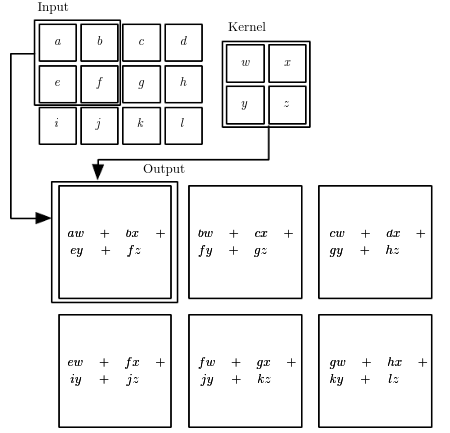
\includegraphics[width=4.5cm]{convolution.png}
\caption{Opération de convolution label:convolution}
\end{figure}
\begin{itemize}
\item entrée : une matrice
\item applique le kernel sur l'entrée
\item sortie : une carte des caractéristiques (feature map)
\end{itemize}
\end{frame}

\begin{frame}[label={sec:orgd665bae}]{CNN : intéraction parcimonieuse}
\begin{figure}[htbp]
\centering
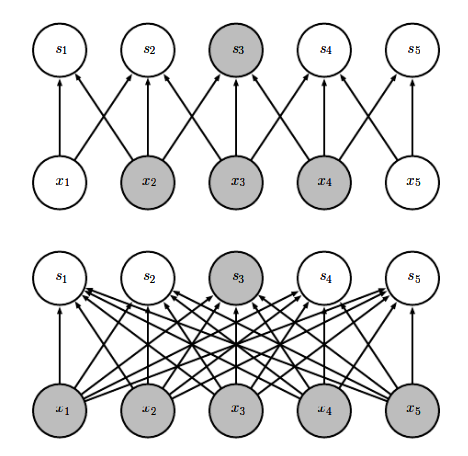
\includegraphics[width=4cm]{sparse_vs_dense.png}
\caption{Intéraction parcimonieuse (en haut), intéraction non parcimonieuse (en bas) label:sparse-vs-dense}
\end{figure}
\begin{itemize}
\item taille kernel < taille entrée
\item le kernel ne parcourt qu'une petite partie de l'entrée à la fois
\item moins de calculs à effectuer
\end{itemize}
\end{frame}

\begin{frame}[label={sec:org83ff5b2}]{CNN : partage de paramètres}
\begin{itemize}
\item un seul kernel itére sur l'entrée de la couche
\item le réseau n'apprend que les poids du kernel
\item taille kernel << taille entrée
\end{itemize}

=> beaucoup moins de paramètres à apprendre
\end{frame}

\begin{frame}[label={sec:orgdee1f1a}]{CNN : pooling}
\begin{figure}[htbp]
\centering
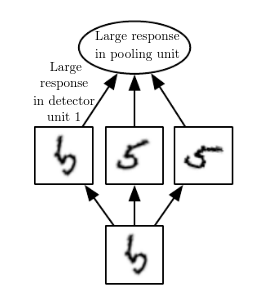
\includegraphics[width=3cm]{pooling.png}
\caption{Pooling \& invariance label:pooling}
\end{figure}

\begin{itemize}
\item modifie la sortie de la couche de convolution
\item fait une approximation de la sortie
\item rend la représentation \alert{invariante} à de petits changements sur l'entrée
\item améliore la capacité de généralisation des CNN
\end{itemize}
\end{frame}

\section{Détection par apprentissage profond}
\label{sec:orge9d0880}
\begin{frame}[label={sec:org2ab2a78}]{Two-Stream Convolutional Networks (1/4)}
Séparation de la tâche de reconnaissance dans les vidéos en 2 parties :
\begin{itemize}
\item composante spatialle
\item composante temporelle
\end{itemize}
Un CNN est associé à chaque composante
\end{frame}

\begin{frame}[label={sec:org0d01a78}]{Two-Stream Convolutional Networks : Composante spatialle (2/4)}
\begin{itemize}
\item Classifieur d'image classique (imageNet, GoogLeNet)
\item Donne un indice fort sur l'action
\item Bénéficie des avancées dans le domaine de l'image
\end{itemize}
\end{frame}

\begin{frame}[label={sec:org519057d}]{Two-Stream Convolutional Networks : Composante temporelle (3/4)}
\begin{figure}[htbp]
\centering
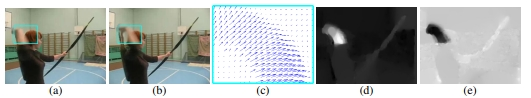
\includegraphics[width=12cm]{optical_flow_slide.jpg}
\caption{Flux optique label:optical-flow label:opt-flow}
\end{figure}
\begin{itemize}
\item utilise l'algorithme de flux optique
\begin{itemize}
\item détecte le mouvement entre les images de la vidéo
\end{itemize}
\item entrée du CNN temporel : image flux optique
\end{itemize}
\end{frame}

\begin{frame}[label={sec:org5561717}]{Two-Stream Convolutional Networks : (4/4)}
\begin{figure}[htbp]
\centering
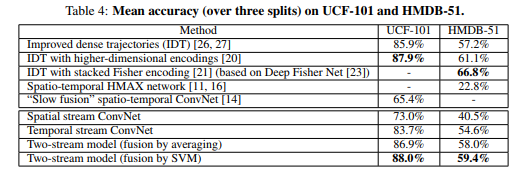
\includegraphics[width=10cm]{two_stream_res.png}
\caption{Résultats obtenus par l'approche Two-stream model label:two-stream-res}
\end{figure}

Apport de la composante temporelle : +15\%
\end{frame}

\begin{frame}[label={sec:org01d863f}]{Réseau à convolution 3D (1)}
\begin{itemize}
\item article Learning Spatiotemporal Features with 3D Convolutional Networks cite:Tran\(_{\text{2015}}\)
\item idée :
\begin{itemize}
\item 2D : image
\item 3D : video = image + temps
\end{itemize}
\item apprendre la temporalité grâce à la convolution 3D
\end{itemize}
\end{frame}

\begin{frame}[label={sec:orgb9bae18}]{Réseau à convolution 3D (2)}
\begin{figure}[htbp]
\centering
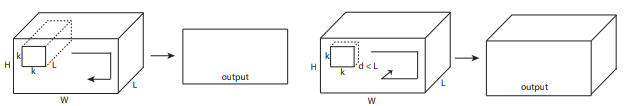
\includegraphics[width=.9\linewidth]{c3d_idea.png}
\caption{Convolution 2D sur une séquence d'image (gauche), convolution 3D sur une séquence d'image (droite) label:c3d-idea}
\end{figure}
\begin{itemize}
\item convolution 2D : produit une image (2D) => perte de l'info temporelle
\item convolution 3D : produit une réprésentation 3D => garde l'info temporelle
\end{itemize}
\end{frame}

\begin{frame}[label={sec:org2057f15}]{Réseau à convolution 3D (3)}
\end{frame}


\section{Suite de la recherche}
\label{sec:org3e2c8ef}
\begin{frame}[label={sec:org5c4537c}]{Objectif}
\begin{itemize}
\item implémenter l'approche par convolution 3D
\item comparer avec l'approche par détection de contours
\end{itemize}
\end{frame}

\begin{frame}[label={sec:orgf20d3a5}]{Référence}
\end{frame}
\begin{frame}[label={sec:org0d8a804}]{Table des figures}
ref:arch-lstm Ng, J. Y., Hausknecht, M., Vijayanarasimhan, S., Vinyals, O., Monga, R., \& Toderici, G., Beyond short snippets: deep networks for video classification, 2015 IEEE Conference on Computer Vision and Pattern Recognition (CVPR), (),  (2015).  \url{http://dx.doi.org/10.1109/cvpr.2015.7299101}. Figure 3

ref:convolution Goodfellow, I., Bengio, Y., \& Courville, A., Deep Learning (2016), : MIT Press. Chapitre 9. Figure 9.1

ref:pooling Goodfellow, I., Bengio, Y., \& Courville, A., Deep Learning (2016), : MIT Press. Chapitre 9. Figure 9.9

ref:opt-flow Simonyan, K., \& Zisserman, A., Two-stream convolutional networks for action recognition in videos, CoRR, abs/1406.2199(),  (2014). Figure 2

ref:two-stream-res Simonyan, K., \& Zisserman, A., Two-stream convolutional networks for action recognition in videos, CoRR, abs/1406.2199(),  (2014). Table 4

ref:c3d-idea Tran, D., Bourdev, L., Fergus, R., Torresani, L., \& Paluri, M., Learning spatiotemporal features with 3d convolutional networks, 2015 IEEE International Conference on Computer Vision (ICCV), (),  (2015).  \url{http://dx.doi.org/10.1109/iccv.2015.510}. Figure 1
\end{frame}

\begin{frame}[label={sec:org2865d5c}]{Articles (1/4)}
\begin{itemize}
\item Weiss, Y., Torralba, A., \& Fergus, R., Spectral Hashing, In D. Koller, D. Schuurmans, Y. Bengio, \& L. Bottou (Eds.), Advances in Neural Information Processing Systems 21 (pp. 1753–1760) (2009). : Curran Associates, Inc.
\item Rublee, E., Rabaud, V., Konolige, K., \& Bradski, G., Orb: an efficient alternative to sift or surf, 2011 International Conference on Computer Vision, (),  (2011).  \url{http://dx.doi.org/10.1109/iccv.2011.6126544}
\item Abd-Almageed, W., Online, simultaneous shot boundary detection and key frame extraction for sports videos using rank tracing, 2008 15th IEEE International Conference on Image Processing, (),  (2008).  \url{http://dx.doi.org/10.1109/icip.2008.4712476}
\item Raventós, A., Quijada, R., Torres, L., \& Tarrés, F., Automatic summarization of soccer highlights using audio-visual descriptors, SpringerPlus, 4(1),  (2015).  \url{http://dx.doi.org/10.1186/s40064-015-1065-9}
\end{itemize}
\end{frame}

\begin{frame}[label={sec:org98ec917}]{Articles (2/4)}
\begin{itemize}
\item Duan, L., Xu, M., Tian, Q., \& Xu, C., Mean shift based video segment representation and applications to replay detection, 2004 IEEE International Conference on Acoustics, Speech, and Signal Processing, (),  (2004).  \url{http://dx.doi.org/10.1109/icassp.2004.1327209}
\item Goodfellow, I., Bengio, Y., \& Courville, A., Deep Learning (2016), : MIT Press.
\item Tran, D., Bourdev, L., Fergus, R., Torresani, L., \& Paluri, M., Learning spatiotemporal features with 3d convolutional networks, 2015 IEEE International Conference on Computer Vision (ICCV), (),  (2015).  \url{http://dx.doi.org/10.1109/iccv.2015.510}
\item Simonyan, K., \& Zisserman, A., Two-stream convolutional networks for action recognition in videos, CoRR, abs/1406.2199(),  (2014).
\end{itemize}
\end{frame}

\begin{frame}[label={sec:org36660f4}]{Articles (3/4)}
\begin{itemize}
\item Farabet, C., Couprie, C., Najman, L., \& LeCun, Y., Learning hierarchical features for scene labeling, IEEE Transactions on Pattern Analysis and Machine Intelligence, 35(8), 1915–1929 (2013).  \url{http://dx.doi.org/10.1109/tpami.2012.231}
\item Lecun, Y., Bottou, L., Bengio, Y., \& Haffner, P., Gradient-based learning applied to document recognition, Proceedings of the IEEE, 86(11), 2278–2324 (1998).  \url{http://dx.doi.org/10.1109/5.726791}
\item Ng, J. Y., Hausknecht, M., Vijayanarasimhan, S., Vinyals, O., Monga, R., \& Toderici, G., Beyond short snippets: deep networks for video classification, 2015 IEEE Conference on Computer Vision and Pattern Recognition (CVPR), (),  (2015).  \url{http://dx.doi.org/10.1109/cvpr.2015.7299101}
\item Pan, H., Li, B., \& Sezan, , Automatic detection of replay segments in broadcast sports programs by detection of logos in scene transitions, IIEEE International Conference on Acoustics Speech and Signal Processing, (),  (2002).  \url{http://dx.doi.org/10.1109/icassp.2002.1004638}
\end{itemize}
\end{frame}
\begin{frame}[label={sec:orgdb83796}]{Articles (4/4)}
\begin{itemize}
\item Chu, W., Song, Y., \& Jaimes, A., Video co-summarization: video summarization by visual co-occurrence, 2015 IEEE Conference on Computer Vision and Pattern Recognition (CVPR), (),  (2015).  \url{http://dx.doi.org/10.1109/cvpr.2015.7298981}
\item Javed, A., Irtaza, A., Khaliq, Y., Malik, H., \& Mahmood, M. T., Replay and key-events detection for sports video summarization using confined elliptical local ternary patterns and extreme learning machine, Applied Intelligence, 49(8), 2899–2917 (2019).  \url{http://dx.doi.org/10.1007/s10489-019-01410-x}
\item Xu, W., \& Yi, Y., A robust replay detection algorithm for soccer video, IEEE Signal Processing Letters, 18(9), 509–512 (2011).  \url{http://dx.doi.org/10.1109/lsp.2011.2161287}
\end{itemize}
bibliography:summary.bib
\end{frame}
\end{document}
